\section{Experiments}
% We should also soon play with the number of prompt examples to see the effect for some/most tasks. That could be a figure.
% It's probably good to check sensitivity to the random prompts you use (unless they're different for each example), since those types of few-shot numbers can be especially noisy / sensitive
% We'll also want one-shot and zero-shot results.
% Include UnifiedQA or Unicorn or T5 results.
% Look at Atari figures for how to present results on tons of tasks on one page.

% In this section, we show results of state-of-the-art language models on our massive multitask benchmark.

% RoBERTa-base attains an overall accuracy of $27.9\%$, with $27.9\%$ accuracy for the humanities, $28.8\%$ for social sciences, $27.0\%$ for STEM, and $27.7\%$ for other. ALBERT-xxlarge attains an accuracy of $27.1\%$, with $27.2\%$ accuracy for the humanities, $25.7\%$ for the social sciences, $27.7\%$ for STEM, and $27.9\%$ for other. GPT-2 attains an accuracy of $32.4\%$, with $32.8\%$ accuracy for the humanities, $33.3\%$ for the social sciences, $30.2\%$ for STEM, and $33.1\%$ for other.

% UnifiedQA: 0.29348675332054835, 0.32353150081681936, 0.38028269053199804, 0.4376731301939058, 0.48938134810710987
\begin{table}[b]
\setlength{\tabcolsep}{9pt}
\vspace{-5pt}
%\scriptsize
%\footnotesize
\fontsize{10}{11}\selectfont
\centering
\begin{tabular}{lcccc|c}
Model       & Humanities & Social Science & STEM & Other &  Average \\
\hline
Random Baseline & 25.0 & 25.0 & 25.0 & 25.0 & 25.0 \\
% T5 & 24.9 & 25.2 & 24.8 & 24.4 & 24.8 \\
% UnifiedQA Small    &  &  &  &  &  \\
% UnifiedQA Base     &  &  &  &  &  \\
% UnifiedQA Large    &  &  &  &  &  \\
RoBERTa           & 27.9 & 28.8 & 27.0 & 27.7 & 27.9 \\
ALBERT           & 27.2 & 25.7 & 27.7 & 27.9 & 27.1 \\
GPT-2           & 32.8 & 33.3 & 30.2 & 33.1 & 32.4 \\
UnifiedQA       & 45.6 & 56.6 & 40.2 & 54.6 & 48.9 \\
GPT-3 Small (few-shot)     & 24.4 & 30.9 & 26.0 & 24.1 & 25.9 \\
GPT-3 Medium (few-shot)   & 26.1 & 21.6 & 25.6 & 25.5 & 24.9 \\
GPT-3 Large (few-shot)     & 27.1 & 25.6 & 24.3 & 26.5 & 26.0 \\
GPT-3 X-Large (few-shot)   & 40.8 & 50.4 & 36.7 & 48.8 & 43.9 \\
\hline
\end{tabular}
% \vspace{2pt}
\caption{Average weighted accuracy for each model on all four broad disciplines. All values are percentages. Some models proposed in the past few months can move several percent points beyond random chance. GPT-3 uses few-shot learning and UnifiedQA is tested under distribution shift.}
\label{tab:mainresults}
% \label{results}
% \vspace{-10pt}
\end{table}


\subsection{Setup}

\paragraph{Assessment and Models.} To measure performance on our multitask test, we compute the classification accuracy across all examples and tasks. We evaluate GPT-3 \citep{brown2020gpt3} and UnifiedQA \citep{khashabi2020unifiedqa}.
For GPT-3 we use the OpenAI API, which provides access to four model variants,  ``Ada,'' ``Babbage,'' ``Curie,'' and ``Davinci,'' which we refer to as ``Small'' ($2.7$ billion parameters), ``Medium'' ($6.7$ billion), ``Large'' ($13$ billion) and ``X-Large'' ($175$ billion). 
%Unless noted otherwise, we evaluate GPT-3 models in a $5$-shot setting.
UnifiedQA uses the T5 \citep{raffel2019exploringT5} text-to-text backbone and is fine-tuned on previously proposed question answering datasets \citep{lai2017race}, where the prediction is the class with the highest token overlap with UnifiedQA's text output. Since UnifiedQA is fine-tuned on other datasets, we evaluate it without any further tuning to assess its transfer accuracy. We also fine-tune RoBERTa-base, ALBERT-xxlarge, and GPT-2 on UnifiedQA training data and our dev+val set. We primarily focus on UnifiedQA and GPT-3 in the rest of this document, but additional discussion of RoBERTa, ALBERT, and GPT-2 is in \Cref{app:additional}.
% model under distribution to our benchmark without task-specific fine-tuning, we evaluate it under distribution shift.

\begin{wrapfigure}{R}{0.5\textwidth}
	\vspace{-5pt}
	\begin{center}
	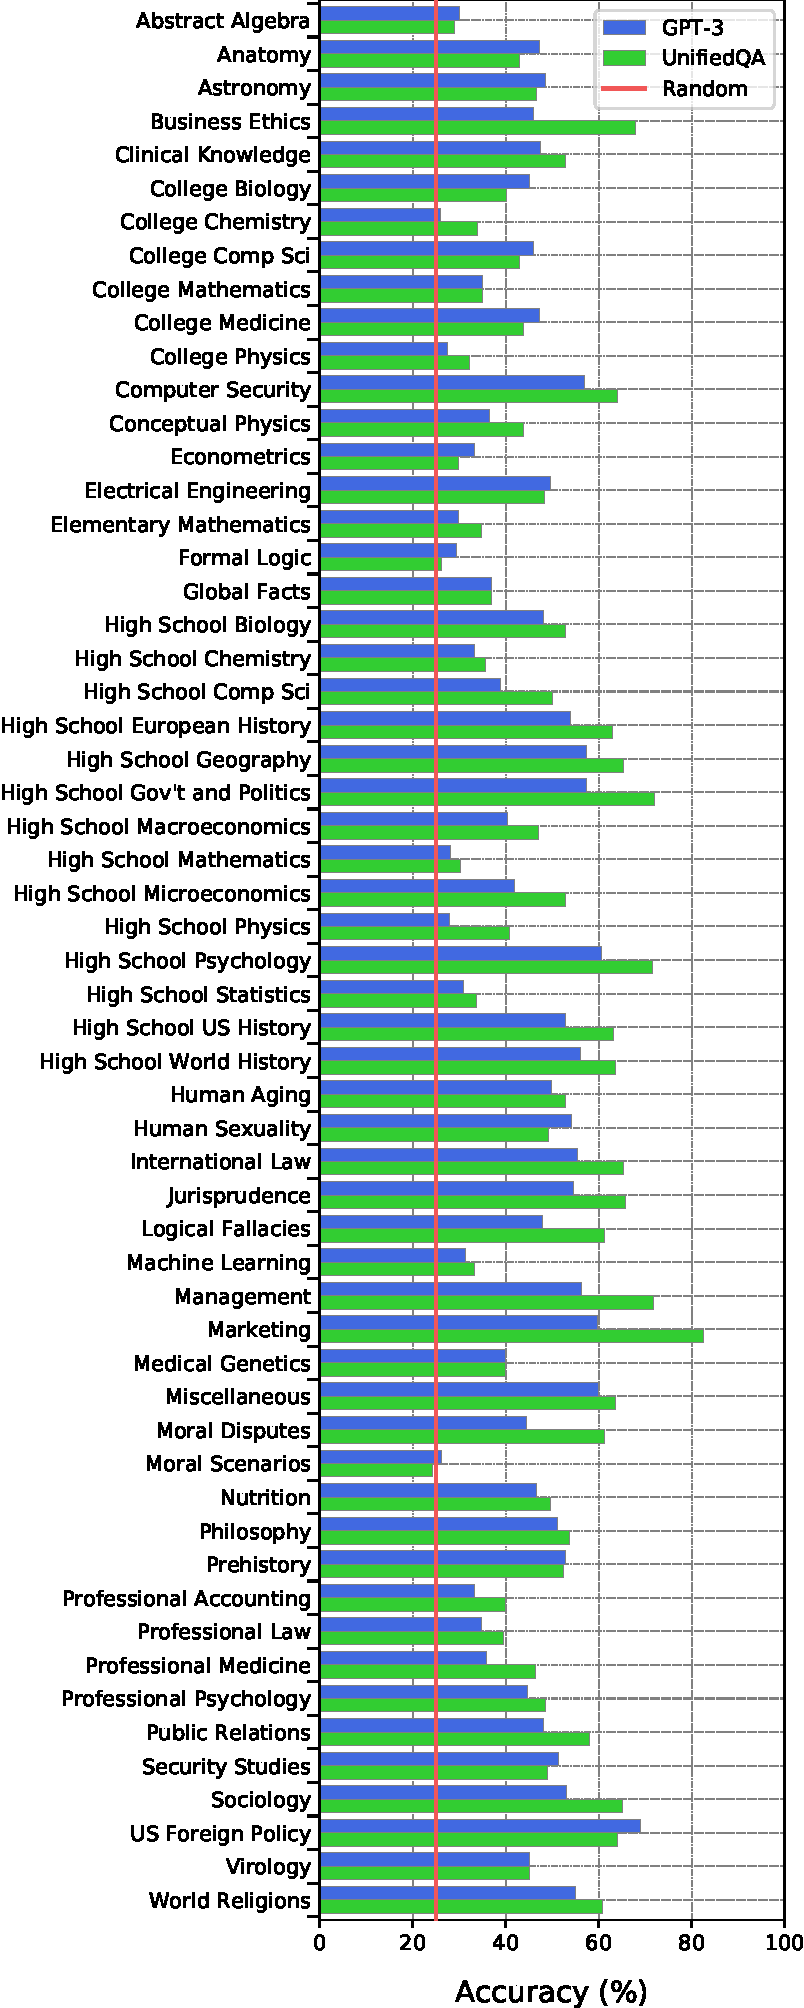
\includegraphics[width=0.5\textwidth]{figures/merged_results.pdf}
	\end{center}
	\vspace{-10pt}
	\caption{
	GPT-3 (few-shot) and UnifiedQA results.
	%GPT-3 few shot accuracies for all of the $57$ tasks. All task accuracies are markedly below expert-level performance.
    }\label{fig:fullresults}
	\vspace{-50pt}
\end{wrapfigure}

\paragraph{Few-Shot Prompt.} We feed GPT-3 prompts like that shown in \Cref{fig:fewshot}. We begin each prompt with ``The following are multiple choice questions (with answers) about [subject].'' For zero-shot evaluation, we append the question to the prompt. For few-shot evaluation, we add up to $5$ demonstration examples with answers to the prompt before appending the question. All prompts end with ``Answer: ''. The model then produces probabilities for the tokens ``A,'' ``B,'' ``C,'' and ``D,'' and we treat the highest probability option as the prediction. %For most subjects, we could add exactly $5$ demonstrations per example, but for a few subjects with long questions we only added as many demonstrations as could fit in the context window of $2048$ tokens.
For consistent evaluation, we create a dev set with $5$ fixed few-shot examples for each subject.

\subsection{Results}

\paragraph{Model Size and Accuracy.}
% while obvious that larger models better, unclear by how much.
%While it is well known that large models generally perform better than small models, how much performance improves with model size varies by task. Evaluating how accuracy scales with the number of parameters can inform us about future performance.
% diminishing returns

We compare the few-shot accuracy of each GPT-3 size in \Cref{tab:mainresults}. We find that the three smaller GPT-3 models have near random accuracy (around $25\%$). %We also assess the $11$ billion parameter T5 model in a few-shot setting and confirmed that it likewise has random chance accuracy.
In contrast, we find that the X-Large $175$ billion parameter GPT-3 model performs substantially better than random, with an accuracy of $43.9\%$. We also find qualitatively similar results in the zero-shot setting. While the smaller models have around $25\%$ zero-shot accuracy, \Cref{fig:kandacc} in \Cref{app:additional} shows that the largest GPT-3 model has a much higher zero-shot accuracy of about $37.7\%$. \citet{brown2020gpt3} also observe that larger GPT-3 models perform better, though progress tends to be steadier. In \Cref{fig:juxtaposition} we show that non-random accuracy on the multitask test emerged with recent large few-shot models compared to datasets that assess commonsense and linguistic understanding.


% This sudden jump in accuracy is distinctly sharp compared to other benchmarks. We illustrate this in \Cref{fig:juxtaposition}, which shows that performance increases much more gradually with model size for HellaSwag and SuperGLUE, datasets that assess commonsense and linguistic understanding.

% To see if this size-accuracy discontinuity holds for other models, we also evaluated UnifiedQA models. 
To test the usefulness of fine-tuning instead of few-shot learning, we also evaluate UnifiedQA models. 
UnifiedQA has the advantage of being fine-tuned on other question answering datasets, unlike GPT-3. We assess UnifiedQA 
% on our distinct test questions 
by evaluating its transfer performance without any additional fine-tuning. The largest UnifiedQA model we test has $11$ billion parameters, which is slightly smaller than GPT-3 Large. Nevertheless, we show in \Cref{tab:mainresults} that it attains $48.9\%$ accuracy. This performs better than the few-shot GPT-3 X-Large model, despite UnifiedQA have an order of magnitude fewer parameters. We also find that even the smallest UnifiedQA variant, with just $60$ million parameters, has approximately $29.3\%$ accuracy.
These results suggest that while model size is a key component for achieving strong performance, fine-tuning also helps.% is not the only important factor.

% These results suggest that some small open-source research models can be competitive with larger proprietary models.

% How to end? What's the takeaway? 
% Larger models indeed important, but they're not everything


% fine-tuning before transferring to a different test distribution can do much better than directly applying a pretrained model in a few-shot setting.

% \begin{figure}[t]
%     \centering
%     % \vspace{-10pt}
%     % 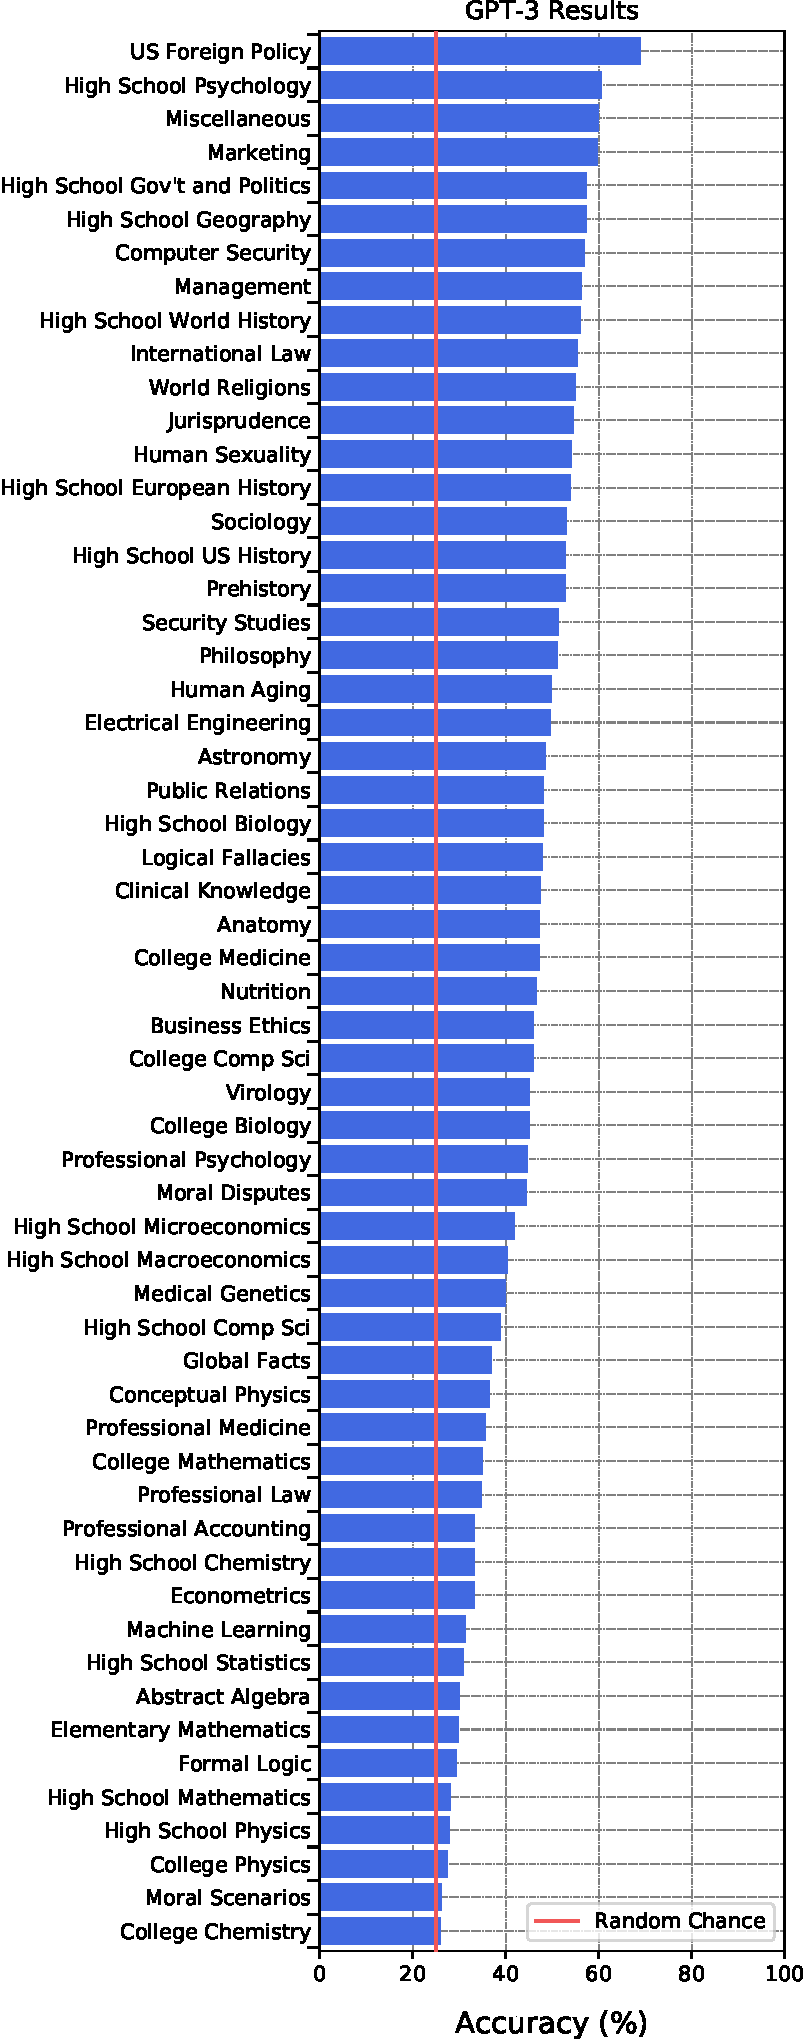
\includegraphics[width=\textwidth]{figures/full_results.pdf}
%     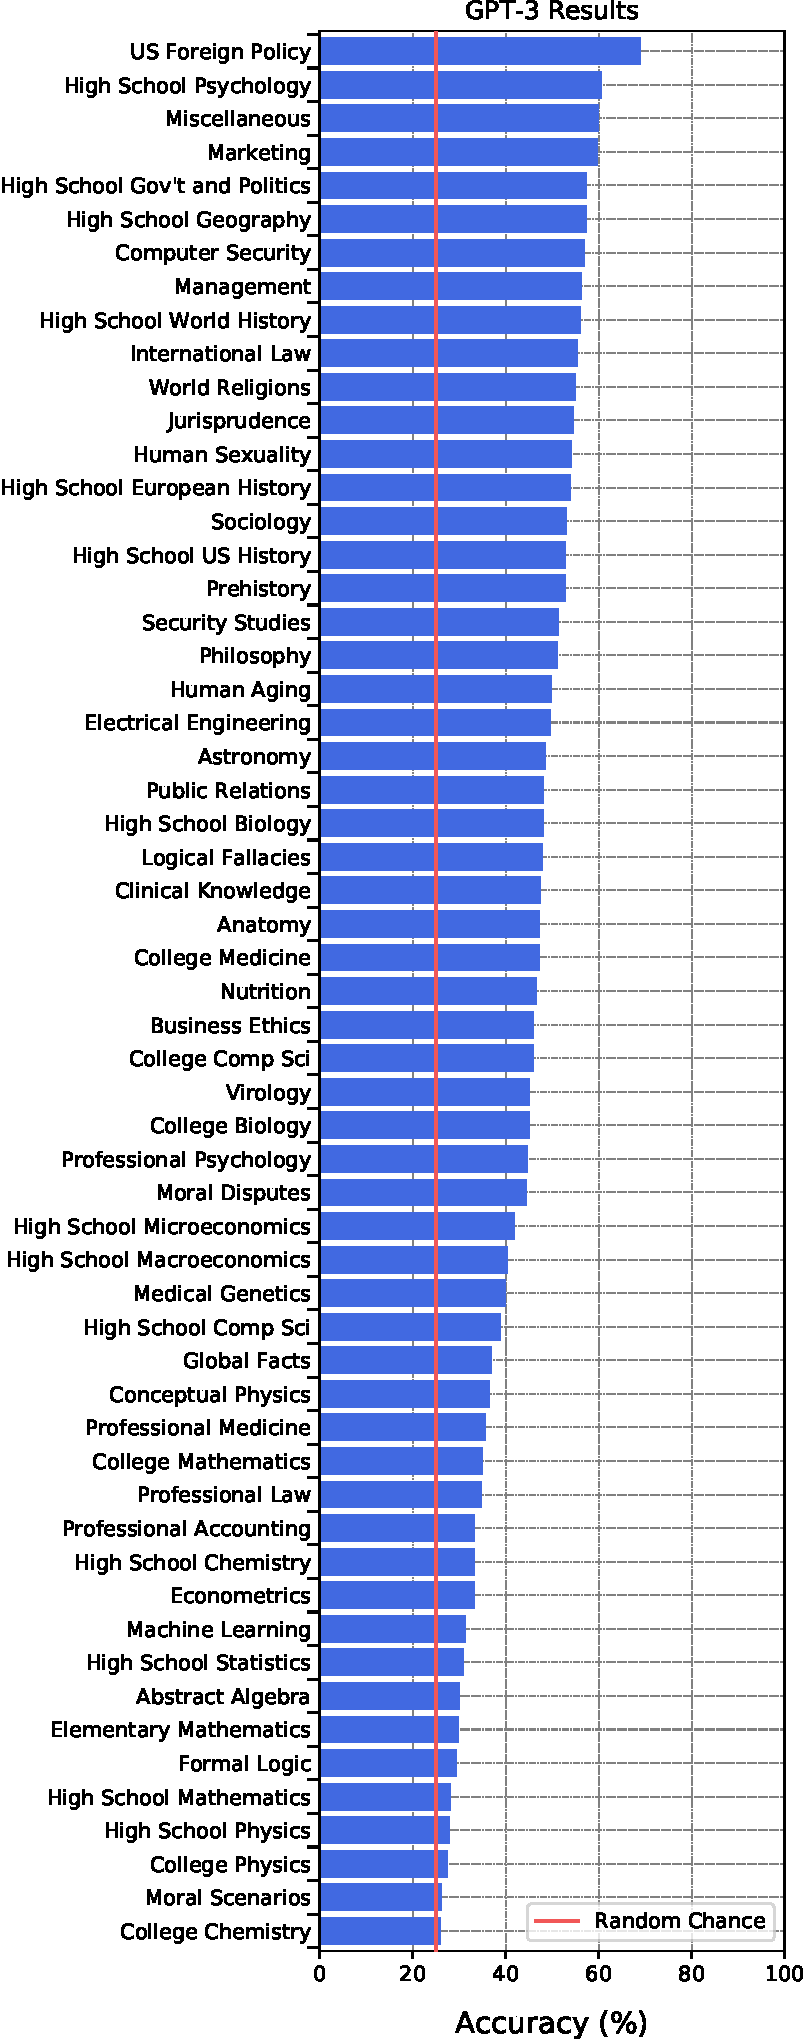
\includegraphics[width=0.5\textwidth]{figures/full_results.pdf}
%     \caption{911
%     \looseness=-1}
%     \label{fig:fullresults}
%     % \vspace{-10pt}
% \end{figure}

\noindent\textbf{Comparing Disciplines.}\quad
Using our test, we discover that GPT-3 and UnifiedQA have lopsided performance and several substantial knowledge gaps. \Cref{fig:fullresults} shows the accuracy of GPT-3 (few-shot) and UnifiedQA for all $57$ tasks. It shows the both models are below expert-level performance for all tasks, with GPT-3's accuracy ranging from $69\%$ for US Foreign Policy to $26\%$ for College Chemistry. UnifiedQA does best on marketing, with an accuracy of $82.5\%$.
% 1. start with conclusion (many gaps)? 
% 2. 


Overall, models do poorly on highly procedural problems.
% The calculation-heavy STEM subjects have low accuracy, and tasks with many ``plug and chug'' problems such as Elementary Mathematics present a greater challenge than verbal subjects such as Professional Psychology. 
\Cref{fig:fullresults} shows that calculation-heavy STEM subjects tend to have low accuracy compared to verbal subjects.
For GPT-3, $9$ out of the $10$ lowest-accuracy tasks are STEM subjects that emphasize mathematics or calculations.
We speculate that is in part because GPT-3 acquires declarative knowledge more readily than procedural knowledge. For example, many questions in Elementary Mathematics require applying the order of operations for arithmetic, which is described by the acronym PEMDAS (Parentheses Exponents Multiplication Division Addition Subtraction). In \Cref{fig:pemdas}, we confirm that GPT-3 is \emph{aware} of the acronym PEMDAS. However, it does not consistently \emph{apply} PEMDAS to actual problems. 
% This suggests GPT-3 is less capable at applying procedures to particular instances. 
On the other hand, procedural understanding is not its only weak point. We find that some verbal tasks such as Moral Scenarios from \cite{hendrycks2020ethicsdataset} and Professional Law also have especially low accuracy.

% \begin{wrapfigure}{R}{0.4\textwidth}
% % \vspace{-10pt}
% \centering
% 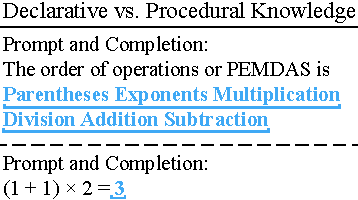
\includegraphics[width=0.4\textwidth]{figures/pemdas.pdf}
% \caption{GPT-3's \textcolor{rightblue}{completion} for two prompts testing knowledge of the order of operations.
% %The \textcolor{rightblue}{blue} underlined bold text is the autocompleted response from GPT-3.
% While it \emph{knows about} the order of operations, it sometimes does not \emph{know how} to apply its knowledge.\looseness=-1% and does not obey operator precedence.
% }\label{fig:pemdas}% Hence for this multitask test, additional prompt examples are only moderately effective at increasing accuracy and are not necessary to escape random-chance accuracy levels.\phantom{Here's some text to make sure the}}\label{fig:kandacc}
% \vspace{-20pt}
% \end{wrapfigure}

Our test also shows that GPT-3 acquires knowledge quite unlike humans. For example, GPT-3 learns about topics in a pedagogically unusual order.
GPT-3 does better on College Medicine ($47.4\%$) and College Mathematics ($35.0\%$) than calculation-heavy Elementary Mathematics ($29.9\%$). GPT-3 demonstrates unusual breadth, but it does not master a single subject. Meanhwhile we suspect humans have mastery in several subjects but not as much breadth. In this way, our test shows that GPT-3 has many knowledge blindspots and has capabilities that are lopsided.


% \begin{wrapfigure}{R}{0.42\textwidth}
% 	\vspace{-10pt}
% 	\begin{center}
%     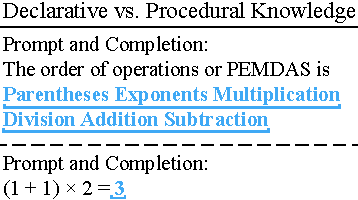
\includegraphics[width=0.42\textwidth]{figures/pemdas.pdf}
%     \caption{GPT-3's completion for two prompts testing knowledge of the order of operations. The \textcolor{rightblue}{blue} underlined bold text is the autocompleted response from GPT-3. While it is has descriptive knowledge and knows \emph{about} of the order of operations, it does not know \emph{how} to apply its knowledge and does not obey operator precedence.}\label{fig:pemdas}% Hence for this multitask test, additional prompt examples are only moderately effective at increasing accuracy and are not necessary to escape random-chance accuracy levels.\phantom{Here's some text to make sure the}}\label{fig:kandacc}



% \begin{wrapfigure}{R}{0.5\textwidth}
% \vspace{-15pt}
% \centering
% 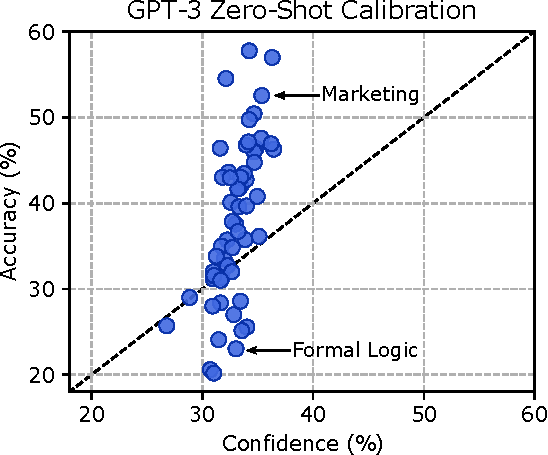
\includegraphics[width=0.5\textwidth]{figures/calibration_arrows.pdf}
% \caption{
% GPT-3's confidence is a poor estimator of its accuracy and can be off by up to $24\%$.\looseness=-1
% %GPT-3's average confidence and accuracy on each subject in a zero-shot setting. Its confidence is a poor estimator of its accuracy and can be off by up to $20\%$.
% }\label{fig:calibration}
% \vspace{-10pt}
% \end{wrapfigure}

\begin{figure}
\vspace{-20pt}
\begin{minipage}{.5\textwidth}
\centering
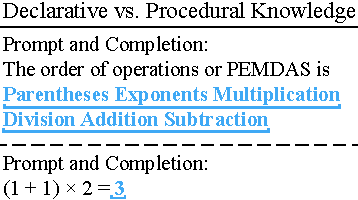
\includegraphics[width=0.9\textwidth]{figures/pemdas.pdf}
\caption{GPT-3's completion for two prompts testing knowledge of the order of operations.
The \textcolor{rightblue}{blue} underlined bold text is the autocompleted response from GPT-3.
While it \emph{knows about} the order of operations, it sometimes does not \emph{know how} to apply its knowledge.\looseness=-1}\label{fig:pemdas}
\end{minipage}%
\begin{minipage}{.5\textwidth}
\centering
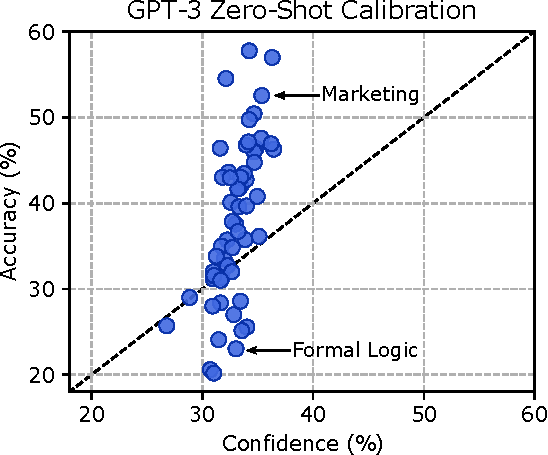
\includegraphics[width=\textwidth]{figures/calibration_arrows.pdf}
\caption{
GPT-3's confidence is a poor estimator of its accuracy and can be off by up to $24\%$.\looseness=-1
%GPT-3's average confidence and accuracy on each subject in a zero-shot setting. Its confidence is a poor estimator of its accuracy and can be off by up to $20\%$.
}\label{fig:calibration}
\end{minipage}
\vspace{-15pt}
\end{figure}

\noindent\textbf{Calibration.}\quad
We should not trust a model's prediction unless the model is calibrated, meaning that its confidence is a good estimate of the actual probability the prediction is correct. However, large neural networks are often miscalibrated \citep{kilian2017calibration}, especially under distribution shift \citep{ovadia2019can}. 
We evaluate the calibration of GPT-3 by testing how well its average confidence estimates its actual accuracy for each subject.
We show the results in \Cref{fig:calibration}, which demonstrates that GPT-3 is uncalibrated. In fact, its confidence is only weakly related to its actual accuracy in the zero-shot setting, with the difference between its accuracy and confidence reaching up to $24\%$ for some subjects.
Another calibration measure is the Root Mean Squared (RMS) calibration error \citep{hendrycks2019oe,kumar2019verifiedcalibration}. Many tasks have miscalibrated predictions, such as Elementary Mathematics which has a zero-shot RMS calibration error of 19.4\%. Models are only somewhat more calibrated in the few-shot setting, as shown in \Cref{app:additional}.
% \dan{Add RMS!!} %We find less dramatic results in the few-shot setting, as shown in \Cref{fig:fewshotcalibration} in \Cref{fig:, but the difference between accuracy and confidence still reaches up to $12\%$ for some subjects.
These results suggest that model calibration has wide room for improvement.


% We measure the calibration of GPT-3 in a few-shot setting. To measure calibration, we use the Root Mean Squared (RMS) calibration error \citep{hendrycks2019oe,kumar2019verifiedcalibration}. We find that the X-Large model has a RMS of $6.6\%$, compared to $8.6\%$ for the Large model and $9.3\%$ for the two smallest models. While calibration is improving, progress is slow and there is still wide room for improvement.

% How to be a bit more negative here?
% Or could just push for its importance.

% ECE or something else?
% plot?

% how much to define (with ECE or whatever). probably not much.
% Temperature scaling doesn't help, even for smaller models [assuming these results still hold; not sure whether to run myself] 



% \collin{Might be worth testing more here. Should also probably have more of a conclusion, but I'm not sure what.}

% I suppose then it's worth noting how it can learn lots of topics out-of-order. It's not good with numbers, but much of later mathematics don't use numbers.

%This further suggests that  models also seems to do worse at subjects requiring more problem solving. 
%Moreover, even among STEM subjects it does better with those that happen to include more conceptual questions, such as computer security and astronomy. \collin{but bad at conceptual physics... Also, it'd be very nice to have more examples per subject so these are less noisy. Right now weird that e.g. high school math harder than college math. I also kind of wish there were a way to know ahead of time that computer security is more conceptual, since you would think that's out of place by default seeing how high its accuracy is.}
% conceptual (vs problem solving) 
% crystallized (vs fluid)
% remembering facts (vs problem solving)
% fewer steps





% \subsection{Calibration}
% \collin{Just writing down what points we should hit on without worrying about anything else for this and the next subsection.}

% A model is said to be calibrated if the confidence it outputs provides a good estimate of the probability it is correct. While neural networks in computer vision are known to be consistently overconfident [], especially on out-of-distribution inputs [], we found that GPT-3 models are well-calibrated even in a few-shot setting. 

% \collin{To do: actually figure out what experiments we want to discuss and how to frame it. Options include confidence vs actual accuracy (somewhat overconfident, especially for smaller models), temp scaling (seems calibrated), ECE (somewhat calibrated). Jacob, do you have thoughts about this? We should also probably describe how things really are essentially random for the smaller models according to many metrics, but not sure where that should go.}

% %In particular, we can use the average confidence of the model on the entire dataset as an estimate of its overall accuracy. When we do this, we find that 

% % In particular, temperature scaling [] is a simple but effective way to calibrate a model's confidences based on. When we applied temperature scaling, we found that adjusting the temperature parameter didn't help, and that $\alpha = 1.0$ was optimal. 

% \collin{To do: run more experiments checking fine-tuned model calibration. Is this a new property of larger models? Or is this a property of few-shot vs fine-tuned?}

% \subsection{Predicting the Discontinuity?}
% A natural question is whether we could predict the discontinuity, such as by using a metric other than accuracy.
% We tested cross-entropy, brier score, average probability, and average rank, and found that the three smaller GPT-3 variants were all equivalent to random across all of these metrics. This suggests that we may not be able to easily predict similar discontinuities in the future.

% \collin{Are there any other ways we should have predicted this? Did UnifiedQA show a similar discontinuity? Might be worth comparing smaller UnifiedQA models to see.}

% \subsection{Error Analysis}
